\chapter{Modeling Methodology}
\label{chap:procedure}
In this chapter, the methodology of the modelling process of the two models will be described.
\section{Procedure for Modelling of Global Model}
\label{sec:globmod}
The global model was created in SIMA RIFLEX, and represents the total dynamic part of the power cable. It was attached to both the seabed and the a point that will behave like the vessel due to the transfer functions provided from Dr. Techn. Olav Olsen. It is assumed that the most severe damage due to fatigue is located at the top of the cable, so that very little attention was borough to the bottom touchdown. The following section will describe how the central properties of the cable were modeled in the global model. 

\subsection{Cable Configuration}
The global model consists of 3 sections with 2 different cross-sections. Section 1 was the lowest part of the cable and was attached to a super node located on the seabed with the cable cross section. The second section was located in the middle of the cable with buoyancy elements. The third section was the upper part of the cable, and it was attached to a super node on the wind turbine floater, with the cable cross section. An illustration of a typical dynamic power cable configuration with the different sections explained can be seen in Figure \ref{fig:globalill}.\newline
\newline 

\begin{figure}[H]
\centering
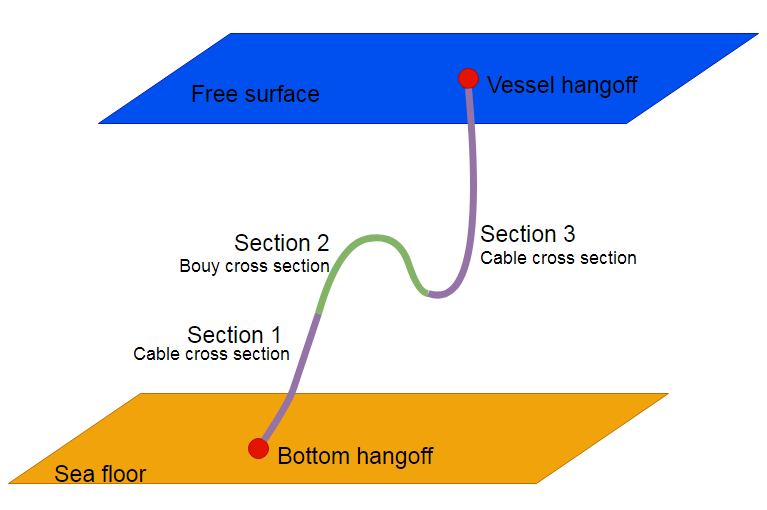
\includegraphics[scale=0.6]{figures/globalill}
\caption [$\; \:$ Illustration of the global model and its different sections ]{Illustration of the global model and its different sections}
 \label{fig:globalill}
\end{figure}
\noindent As a simplification, it was assumed that the floating wind turbine could only have 3 different positions:
\begin{itemize}
    \item Neutral: There is no wind
    \item Near: Maximum wind from the east direction
    \item Far: Maximum wind from the west direction
\end{itemize}
See Section \ref{sec:current} for more detailed information on the weather conditions at each position. \\\\
To determine the far position, it was decided in agreement with Dr. Techn. Olav Olsen that the maximum offset in far position, relative to the Neutral position was 20\% of the water depth in the east direction. Assuming a linear system, the offset in Near position relative to the Neutral position was calculated by using the scatter diagram for wind in Figure \ref{fig:scatterwind}:
\begin{equation}
    \text{Offset Near}=\left(\frac{\text{Max  wind speed from east}}{\text{Max wind speed form west}}\right)^2 \cdot \text{Offset far}
\end{equation}

\noindent The near position was set to be 60 m away from the anchoring, in agreement with Professor Svein Sævik, and the Neutral and Far positions were calculated from by adding the offsets as described above. This gave the following positions: 
\begin{table} [H]
\centering
\begin{tabular}{ |c|c|}
\hline
Position & Distance from anchoring in x-direction [m] \\
 \hline
 \hline
 
Near & 60\\

Neutral & 73.25\\

Far & 96.85 \\
 
 \hline
\end{tabular}
\caption{Floater positions at different wind conditions}
\label{table:pos}
\end{table}

\noindent The final cable configuration was determined by an iterative process, testing numerous different combinations of different lengths for the three sections to achieve with max curvature criteria of 1.3675 $\frac{1}{m}$ calculated from \cite{API2014}, and no tension throughout the cable for neither of the three positions. The final values are displayed in Table \ref{table:DIMCABLE} 
\begin{table} [H]
\centering
\begin{tabular}{ |c|c|c|}
\hline
Section number & External area [m$^2$] & Length [m] \\
 \hline
 \hline
1 & 0.006171 & 30\\
2 & 0.03 & 40\\
3 & 0.006171 & 130\\
 \hline
\end{tabular}
\caption{Dimensions of different sections of cable}
\label{table:DIMCABLE}
\end{table}

\subsection{Cross Sectional Properties}
The properties of the two cable cross sections are presented in Table \ref{table:crosssima}, and Figure \ref{fig:globalill} illustrates the use of the two cross sections.

\begin{table} [H]
\centering
\begin{tabular}{ |c|c|c|}
\hline
Property& Cable Cross Section & Buoy Cross Section \\
 \hline
 \hline
Dry mass+ Buoyancy [$\frac{kg}{m}$] & 15.75 & 15.75\\
External Area [m]& 0.006171 & 0.03\\
Axial Stiffness [N] & 2.0e+08 & 2.0e+08\\
Bending Stiffness [Nm$^2$] & 1481 & 1481\\
Torsional Stiffness [Nm$^2$] & 5403 & 5403\\
 \hline
\end{tabular}
\caption{Parameters used for the two different cross sections}
\label{table:crosssima}
\end{table}
\noindent The only difference between the two cross section types was the external area due to the buoyancy elements attached to the buoy section. The values in Table \ref{table:crosssima} were calculated as follows:\newline
\newline 
\noindent The Dry mass + Buoyancy: 
\begin{equation}
\text{Dry mass + Buoyancy}=L_{c} A_cn_c (\rho_c-\rho_w) + L_{s,1} A_{s}n_{s,1} (\rho_s-\rho_w)+L_{s,2} A_{s}n_{s,2} (\rho_s-\rho_w)
\end{equation}

\noindent where $L_c$ is the length of a helical copper conductor pr meter, $A_c$ is the area of a copper conductors, $n_c$ is the number of copper conductors, $\rho_c$ is the density of copper, $\rho_w$ is the density of water, $L_{s,i}$ is the length of steel armouring pr meter for layer i, $A_s$ is the area of one wire for the steel armouring assumed to be the same for layer 1 and 2, $n_{s,i}$ is the number of wires in armouring layer i and $\rho_s$ is the density of steel. The plastic sheaths and tape were assumed to have the same density as the water, and thus have neutral buoyancy. \newline
\newline 
The axial stiffness and torsional stiffness were calculated according to Equation 4.14 and 4.22 in \cite{Savik2016} as:
\begin{equation}
    EA=nEA_t \cos\alpha(\cos^2\alpha-\nu_a \sin^2\alpha)
\end{equation}

\begin{equation}
    GI=nA_t E R^2 \sin^2 \alpha \cos^2 \alpha
\end{equation}
where $n$ is the number of wires in the steel armouring, $E$ is Young's modulus of steel, $A_t$ is the area of one steel wire, $\alpha$ is the lay angle of the armouring, R is the radius in polar coordinates between the armouring layers.  \newline
\newline 
The bending stiffness was calculated from the outer sheath as follows:
\begin{equation}
    EI= E\cdot \frac{\pi}{4}(r_o-r_i)
\end{equation}
Where E is Young's modulus of the plastic of the outer sheath, $r_o$ is the outer radius of the outer sheath, and $r_i$ is the inner radius of the outer sheath. \newline
\newline 
To increase the weight of the cable and thus increase the inertia, lead was added to the model. According to Professor Svein Sævik, the following criteria would be beneficial for the cable:
\begin{equation}
    \frac{\sum_{i=1}^n m_i - b}{b}\approx 2
\end{equation}
Where $m_i$ is the mass of the different components in the cross section, and b is the buoyancy. To achieve this, 6kg had to be added to the cross section. This was done by making the center tube out of lead, and also place three tubes the size of the center tube in the free space between the conductors and the sheath. To model this, the mass coefficient was increased by 6 kg and reached 15.75 $\frac{kg}{m}$ as shown in Table \ref{table:DIMCABLE}. \newline
\newline A dummy super node was added to the vessel with a dummy line between the two super nodes attached to the vessel. This way it was possible to take the dot product of the dummy line and the upper element of the cable and get a time series of the angle between the vessel and the cable.

\subsection{Boundary Conditions}
The cable was fixed to the seabed in all translational and rotational degrees of freedoms. The cable hang-off on the vessel was fixed in all translational degrees of freedom and free in all rotational degrees of freedom. 

\subsection{Testing of Global Model}
To make sure the global model was ready to be used in further analyses, several things were verified.  The most severe sea state according to the scatter diagram for West of Barra in Figure \ref{fig:scatn} was tested in a dynamic analysis. The key variables used in the test are displayed in Table \ref{table:testglob}.

\begin{table} [H]
\centering
\begin{tabular}{ |c|c|c|}
\hline
Variable & Value \\
 \hline
 \hline
Hs [m] & 13.5\\
Tp[s] & 16 \\
Time step [s] & 0.1 \\
 \hline
\end{tabular}
\caption{Key variables used in testing of global model}
\label{table:testglob}
\end{table}

The following results for the three wind conditions were seen as interesting to assess the quality of the model:
\begin{itemize}
    \item The static configuration without current, to make sure the cable had the desired steep S shape, and that the buoyancy section was not too high in the water.
    \item Curvature envelope, to make sure the curvature did not exceed the max curvature of 1.3675 $\frac{1}{m}$
    \item Max force envelope, to make sure the tension in the cable was acceptable
    \item Min force envelope, to make sure the there was no compression in the bottom of the cable
\end{itemize}
The testing showed that there was no compression in the cable that the curvature did not exceed it criteria. \\\\  The max capacity of the cable was calculated by Equation \ref{eq:tcap} to be 223kN, while the max tension in the cable in static configuration was around 17kN, well within the tension capacity.
\begin{equation}
    T_{cap}=n \cos{(\alpha)} \sigma_y A_s
   \label{eq:tcap}
\end{equation}
where n is the total number of armouring layers in both layers, $\alpha$ is the lay angle, $\sigma_y$ is the yield stress of steel and $A_s$ is the area of one steel fibre.\\\\ 
Based on the results from the testing, it was decided that the global model performed in a satisfactorily manner. All the results were plotted and can be investigated further in Appendix.  \ref{appendix:A}. \newline
\newline
The global model with its three different wind conditions in static configuration without current are shown in Figure \ref{fig:statcon} and Figure \ref{fig:statconc}. 
\begin{figure}[H]
\subfloat[Near position\label{fig:cavS200}]
  {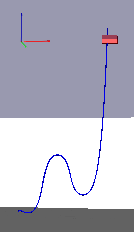
\includegraphics[width=.3\linewidth]{figures/statposnear}}\hfill
\subfloat[Neutral position \label{fig:cavS2500}]
  {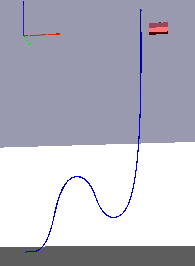
\includegraphics[width=.3\linewidth]{figures/statposneu}}\hfill
  \subfloat[Far position \label{fig:cavS5000}]
  {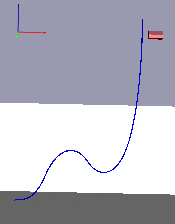
\includegraphics[width=.3\linewidth]{figures/statposfar}}\hfill
\caption{Static configuration for the global model for different wind conditions, without current}
\label{fig:statcon}
\end{figure}

The static configuration with current for the three different wind conditions: 
\begin{figure}[H]
\subfloat[Near position\label{fig:cavS200}]
  {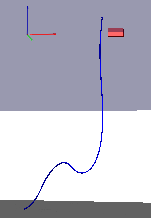
\includegraphics[width=.3\linewidth]{figures/statposnearc}}\hfill
\subfloat[Neutral position \label{fig:cavS2500}]
  {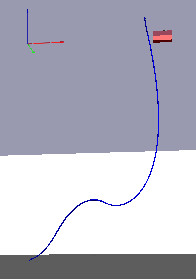
\includegraphics[width=.3\linewidth]{figures/statposneuc}}\hfill
  \subfloat[Far position \label{fig:cavS5000}]
  {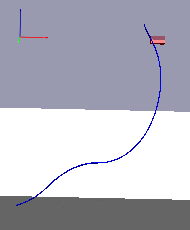
\includegraphics[width=.3\linewidth]{figures/statposfarc}}\hfill
\caption{Static configuration for the global model for different wind conditions, with current}
\label{fig:statconc}
\end{figure}

\section{Procedure for Modelling of Local Model}
\label{sec:localmodel}
The local model was created in BFLEX and consisted of the upper part of the cable, as it was assumed that the most severe fatigue damage occurs here. The model was built up from the inner layer and outwards. It consists of mainly 3 different components as illustrated in Figure \ref{fig:localmod}.
\begin{figure}[H]
\centering
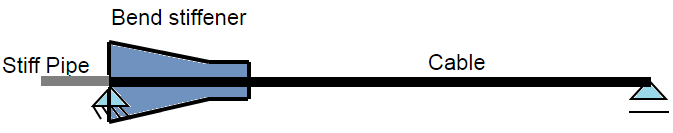
\includegraphics[scale=0.7]{figures/localmod.png}
\caption [$\; \:$Illustration of local model]{Illustration of local model}
 \label{fig:localmod}
\end{figure}
The extra lead added to increase the mass discussed earlier in this chapter was not included in the local model, as it does not have any structural significance other than increasing the mass of the cable.\newline
\newline
\subsection{Cable}
The cable cross section is illustrated in Figure \ref{fig:crosspro}
\begin{figure}[H]
\centering
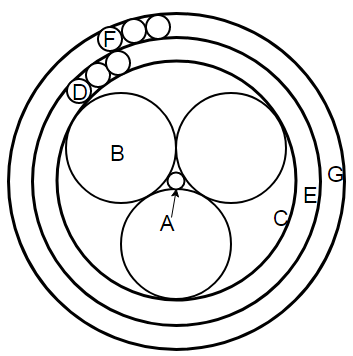
\includegraphics[scale=0.8]{figures/cross2}
\caption [$\; \:$ Cable cross section in local model]{Illustration of cable cross section in local model}
 \label{fig:crosspro}
\end{figure}
\noindent The cable initially consisted of the upper 5 pitch lengths of the cable. However, after running a few analyses it turned out that the model was somewhat short, and it gained some extra length making it 4.25m. It was made up by several layers, as displayed in Figure \ref{fig:cross2}.  The straight components were modeled with HSHEAR363 elements. That includes the center tube (A), the sheath around the conductors (C), the tape between the armouring layers (E), and the outer sheath(G). The helical components were modeled with HSHEAR353 elements and include the conductors (B) and the armouring layers (D) and (F). The cable was built out of one central node system, and all the components were connected to this node system in addition to having their own radial node system.\\\\ To model the contact between element groups, contact elements were used. HCONT463 was used to describe the contact between different layers. The purpose of this element is connecting two other elements, making one of them the master and the other the slave. The modeling started in the inner layer of the cross section, the center tube, and this was the first master element. The element connected the radial node of the core to the radial nodes of the conductors. Then the conductors were the master element and sheath 1 was the slave element. This continued until the outer sheath was reached. An illustration of how the different layers were connected to each other by the HCONT463 is shown in Figure \ref{fig:contact}

\begin{figure}[H]
\centering
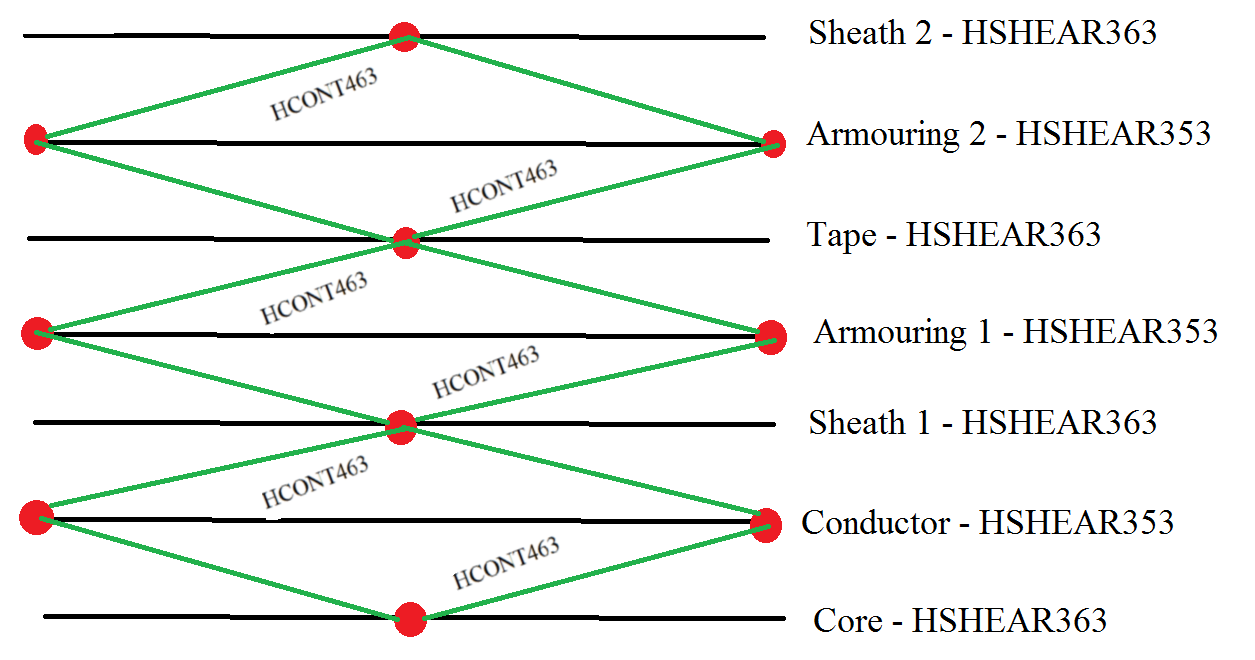
\includegraphics[scale=0.5]{figures/contact}
\caption[$\; \:$ Logic of HCONT463]{The element types for the different components in the cross section and the logic of connecting them by HCONT463}
 \label{fig:contact}
\end{figure}

\noindent To describe the contact between the conductors, the element HCONT454 was used. This element connects the two radial nodes of the HSHEAR353 elements together.\newline
\newline
The conductors were modeled with a lay angle of 8 degrees, and the armouring with a lay angle of 20 degrees according to Professor Svein Sævik's recommendations. \newline
\newline
The cable included three different materials, where the conductors were of copper, the armouring were of steel and the sheaths and tape were made of plastic. The material properties were decided in agreement with Professor Svein Sævik, and the most important material properties are reproduced in Table \ref{table:matprop}
\begin{table} [H]
\centering
\begin{tabular}{ |c|c|c|c|}
\hline
Property &Steel & Copper  & Plastic \\
 \hline
 \hline
Type & Linear & Linear & Elastic\\
Young's modulus [GPA] & 210 & 115 & 0.7\\
Shear modulus [GPA]& 80 & 40 &  \\
Poisson's number [-]& 0.30 & 0.36 & 0.35\\
Axial stiffness [N]& 1.48e+06 & 1.07e+07 & \\
Bending stiffness [Nm$^2$] & 0.835 & 4.19 &\\
Torsional stiffness & 0.64 & 0.32&\\
 \hline
\end{tabular}
\caption{Properties of the materials used in the local model}
\label{table:matprop}
\end{table}


\noindent The friction between layers were determined by the use of FRICONTACT materials. Three different friction models (FRICONTACT materials) were used to model the friction between the layers. The friction properties for each of the friction models are shown in Table \ref{table:friprop}. Table \ref{table:frimod} shows which friction models are used for the contact between the different layers.  

\begin{table} [H]
\centering
\begin{tabular}{ |c|c|c|c|}
\hline
Property &contact01 & contact1  & contact10 \\
 \hline
 \hline
Type & Coulomb friction & Coulomb friction & Coulomb friction\\
Static friction coeff. [-] & 0.15 & 0.15 & 0.15\\
Dynamic friction coeff. [-] & 0.15 & 0.15 & 0.15\\
Elastic stiffness in axial direction $[N/m^$^2$]$ & 100e6 & 100e6 & 100e6 \\
Elastic stiffness in transv. direction $[N/m^$^2$]$& 100e6 & 100e6 & 100e6 \\
Surface stiffness [N/m$^2$] & 100e5 & 100e6 & 100e8\\
 \hline
\end{tabular}
\caption{Properties of the friction elements used in the local model}
\label{table:friprop}
\end{table}

The different friction models for the different contacts are described in Table \ref{table:frimod}

\begin{table} [H]
\centering
\begin{tabular}{ |c|c|}
\hline
Contact & Friction Model  \\
 \hline
 \hline
Core - Conductor & contact01\\
Conductor - Conductor & contact1\\
Conductor - Sheath & contact1\\
Sheath 1 - Armouring 1 & contact1\\
Armouring 1 - Tape &contact10\\
Tape - Armouring 2 &contact10\\
Armouring 2 - Sheath 2 & contact1\\
 \hline
\end{tabular}
\caption{Friction models for different contacts in cable}
\label{table:frimod}
\end{table}

\subsection{Bend Stiffener}
To make the transition in stiffness at the cable hang off smoother, hence adding more local stiffness to the flexible cable, a bend stiffener was added to the model. The following section is based on guidance from Professor Svein Sævik. 
\newline 
\newline
The dimensions of the bend stiffener were roughly calculated in the beginning by the following procedure: \newline
\newline

\noindent Locking radius of the flexible cable:
\begin{equation}
    LR = \frac{r}{1-F_j} = \frac{r}{1-0.9} = 10r
\end{equation}
Where LR is the locking radius, r is the radius of the conductor, $F_j$ is the fillfactor = 0.9 according to professor Svein Sævik. \newline
\newline
Minimum bend radius from \cite{API2014}:
\begin{equation}
   r_{min}= 1.5 * 1.1 * LR
\end{equation}
Where $r_{min}$ is the minimum locking radius, and LR is the locking radius. 
\newline
\newline
Max curvature:
\begin{equation}
   \kappa_{max}= \frac{1}{r_{min}}
\end{equation}
Where $\kappa_{max}$ is the maximum curvature, and  $r_{min}$ is the minimum locking radius.
\newline
\newline
Angle between cable and vessel: 
\begin{equation}
   \theta_{tot} = \theta_{s} + \theta_{p} +   \theta_{offset}
\end{equation}
Where $\theta_{tot}$ is the total angle at the end of the flexible cable, $\theta_{s}$ is angle due to surge, $\theta_{p}$ is angle due to pitch and $\theta_{offset}$ is the angle due to the offset of the floater. These variables are calculated as follows:\newline
\newline 
Angle due to surge:
\begin{equation}
   \theta_{s} = \arctan{(\frac{\mu_{surge}}{L_{1}})}
\end{equation}

\begin{equation}
   \mu_{surge} = \frac{H_{max}}{2} RAO
\end{equation}
Where L{1} is the assumed length from the vessel to the curve on the lazy wave configuration due to the buoyancy elements.  $H_{max}$ is the significant wave height for the most extreme sea state in the scatter diagram in Figure \ref{fig:scatn} and RAO is the response amplitude operator for surge provided by Dr. Techn. Olav Olsen. \newline
\newline 
\noindent Angle due to pitch:
\begin{equation}
   \theta_{pitch} = \frac{H_{max}}{2} RAO
\end{equation}
Where $H_{max}$ is the significant wave height for the most extreme sea state in the scatter diagram in figure \ref{fig:scatn} and RAO is the response amplitude operator for pitch provided by Dr. Techn. Olav Olsen. \newline
\newline
Angle due offset:
\begin{equation}
   \theta_{offset} = \arctan{(\frac{offset * depth}{L_1})}
\end{equation}
This can be used to calculate the length of the bend stiffener:

\begin{equation}
   L_{BS} = \frac{\theta_{max}}{\kappa_{max}} 
  \end{equation}
Where $L_{BS}$ is the length of the bend stiffener, $\theta_{max}$ is the maximum angle and $\kappa_{max}$ is the maximum curvature. \newline
\newline
Further, the outer diameter for the widest part of the bend stiffener can be calculated as follows: \newline
\newline 
Max tension is estimated to 
\begin{equation}
   T = 1.3  T_{static}
\end{equation}
Where T is the max tension, and $T_{static}$ is the static tension due to the configuration of the riser.

\begin{equation}
   T_{static} = 10 + W_s + L_1
\end{equation}
Where $W_s$ is the submerged weight of the cable and $L_1$ is the depth from the floater to the curve on the lazy wave configuration due to the buoyancy elements.\newline
\newline
\noindent $W_s$ was calculated for all the components pr meter cable the following way:

\begin{equation}
   W_s = \sum V (\rho_{comp}-\rho_{water})
\end{equation}
 Where V is the volume for each component, $\rho_{comp}$ is the density of the material of the component and $\rho_{water}$ is the density of the water.\\\\ Number of armouring fibres that fit around the cross section, the following method was used: 

 \begin{equation}
   F_j=\frac{n D}{\cos{(\alpha)} 2 \pi R}
\end{equation}
Where $F_j$ is the fill factor, n is the number of armouring fibers with diameter D  that can fit around a larger circle with radius R, and $\alpha$ is the lay angle of the armouring fibers.  \newline
\newline 
The bending stiffness EI was calculated by the following expression:

 \begin{equation}
   \kappa_{max} = \sqrt{\frac{T_{max}}{EI}}\theta_{max}
\end{equation}
Where $\kappa_{max}$ is the maximum curvature, $T_{max}$ is the maximum tension, EI is the bending stiffness, and $\theta_{max}$ is the maximum angle.\newline  
\newline 
\noindent Finally, the outer radius of the bend stiffener was calculated by:

 \begin{equation}
  EI = \frac{\pi}{4}(r_o^4 - r_i^4) 
\end{equation}
 Where EI is the bending stiffness, $r_o$ is the outer radius of the bend stiffener and $r_i$ is the inner radius.\newline 
\newline 
It turned out that this rough calculation was not quite satisfying, and that the bend stiffener lacked both some length was too wide. With the above calculations as a base, an iterative process was used to improve the dimensions of the bend stiffener. This gave the final dimensions: 
 \begin{table} [H]
\centering
\begin{tabular}{ |c|c|}
\hline
Parameter & Value [m] \\
 \hline
 \hline
 
 Length & 1.400 \\
 
Outer diameter, widest part & 0.260\\

Outer diameter, narrowest part & 0.100\\

 Inner diameter & 0.097 \\
 

 \hline
\end{tabular}
\caption{Dimensions of bend stiffener}
\label{table:dim}
\end{table}
\noindent The bend stiffener begins 1 pitch length away from the upper end of the local model. It was modeled by the use of CROSSECTION command in BFLEX making the inclination very easy to model.  

\subsubsection{Material Data for Bend Stiffener}
The material of the bend stiffener is a polyurethane with non-linear material properties.The initial Young's modulus was chosen to be 150 GPa, with a decay in stiffness according to  Figure \ref{fig:matbend}. The material was chosen in agreement with guidance from Professor Svein Sævik. 

\begin{figure}[H]
\centering
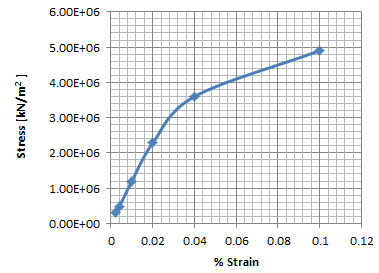
\includegraphics[scale=0.8]{figures/matbend}
\caption[$\; \:$ Stress-strain relationship for bend stiffener material]{Stress-strain relationship for bend stiffener material}
 \label{fig:matbend}
\end{figure}

\subsection{Stiff Pipe}
A stiff pipe was modeled at the very end of the cable. This was done to make sure that there was no curvature in the termination of the cable to avoid transient effects. The pipe had the length of one pitch length and was modeled with PIPE31 elements. The first node of the stiff pipe was connected to the first node of the central node system of through the CONSTR card in BFLEX. The card assigns one node to be the slave and the other to be master, and defines the relationship between them:
\begin{equation}
r_{Si}=C_1 \cdot r_{Mj}    
\end{equation}
Where $r_{Si}$ is the displacement of the slave node,  $C_1$ is a constant describing the relationship between the master and the slave and $r_{Mj}$ is the displacement of a master node.\newline 
\newline 
In this case $C_1$ was 1, so the nodes followed each other exactly. 

\subsection{Method for Application of Tension}
\noindent For easy application of dynamic tension to the model, an extra pipe element was added in the end of the model as can be seen in red in Figure \ref{fig:exelem}. This element had a very low EA, but the same EI as the steel armoring. The purpose of this was to make it possible to apply the tension in the form of strain so that:
\begin{equation}
    \epsilon_0 = T_0
\end{equation}
where $\epsilon_0$ is the reference value for strain and $T_0$ is the reference value for tension. This was scaled so that the reference value was $T_0=$1kN, and desired tension could easily be applied in BFLEX by multiplying the strain with a factor. 
\begin{figure}[H]
\centering
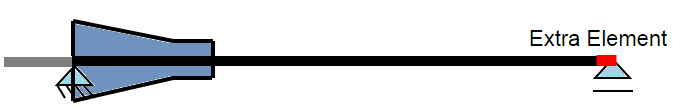
\includegraphics[scale=0.8]{figures/exelem}
\caption[Illustration of the extra element added for easy application of tension]{Illustration of the extra element added for easy application of tension}
 \label{fig:exelem}
\end{figure}

\subsection{Boundary Conditions}
The boundary conditions for the cable was created in such a way that the cable could slide inside the bend stiffener. The following constraints were made for the different components:
\begin{itemize}
    \item Centroid system: Fixed in 2 and 6 for all nodes, and 2 and 3 for the last nodes
    \item Radial nodes of the core, sheaths, and tape are fixed in 2 and 3 for all nodes. 
    \item The conductors are fixed in 1 and 2 for the first and last node. Degree of freedom 4 is fixed in all nodes.
    \item The armouring layers are fixed in 1 at the first node, and in 2,4,5 and 6 for all nodes
\end{itemize}

\subsection{Testing of Local Model}
\label{sec:localtest}
The local model was, as the global model, tested to see if it performed in a satisfactorily manner.
 \noindent The following sequence of loads was added to the local model:
\begin{enumerate}
    \item Gravity Load: Gravity was turned off on the local model, but the effect of the mass of the model had to be applied. This was added at the very first time step.
    \item Tension: The mean tension was added to the local model in the axial direction on the last node in the outer sheath, with magnitude 13.7kN found by the global analyses. The load was applied at t=1s to t=5s. seconds
    \item Initial strain: Initial strain was added to the outer sheath of the model in 1 direction. The strain was added to all the elements with a magnitude 0.03. It was applied at t=1s to t=5s.
    \item Bending: Smooth bending of the cable was applied. The cable was bent from 0 degrees to 5 degrees between t=5s and t=15s, and from 5 degrees to -5 degrees between t=15s and t=35s.  
\end{enumerate}
The following results were seen as interesting when assessing the local model:
\begin{itemize}
    \item Force in the conductors over the length of the cable
    \item Moments about X,Y and Z axis over the length of the cable
    \item Curvature of the outer sheath over the length of the cable
    \item Curvature in bend stiffener
\end{itemize}
The testing showed that the local model was acceptable. All the results for the testing of the local model can be seen in Figures \ref{fig:bflexax} to \ref{fig:bendstiff} in Appendix \ref{appendix:B}. Figure \ref{fig:bflexax} shows that the tension variation on the conductors between max angle and min angle died out towards the end of the model, indicating that the model was of sufficient length, and the same can be seen for the moments in Figure \ref{fig:bflexmx} to Figure \ref{fig:bflexmz}. The curvature is about zero at the beginning and end of the outer sheath (Figure \ref{fig:bflexcurve}), and the bend curvature in the bend stiffener (Figure \ref{fig:bendstiff}) has the desired shape. This indicates that the bend stiffener had appropriate dimensions and was serving its purpose. \\\\
Figure \ref{fig:local1} and Figure \ref{fig:local2} show the actual local model and some of its components as they looked in XPOST.

\begin{figure}[H]
\subfloat[Local model from the side with bend stiffener \label{fig:lm_total}]
  {
\includegraphics[width=.45\linewidth]{figures/lm_total}}\hfill
\subfloat[Cable cross section in local model \label{fig:lm_cross}]
  {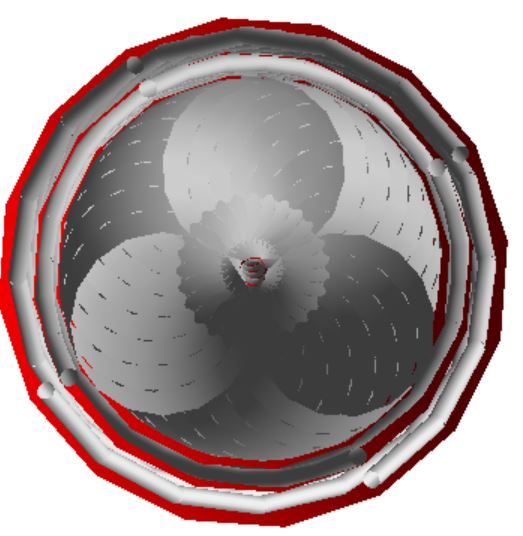
\includegraphics[width=.25\linewidth]{figures/lm_cross}}\hfill
\caption{Local model}
\label{fig:local1}
\end{figure}

\begin{figure}[H]
\subfloat[Conductors \label{fig:single}]
  {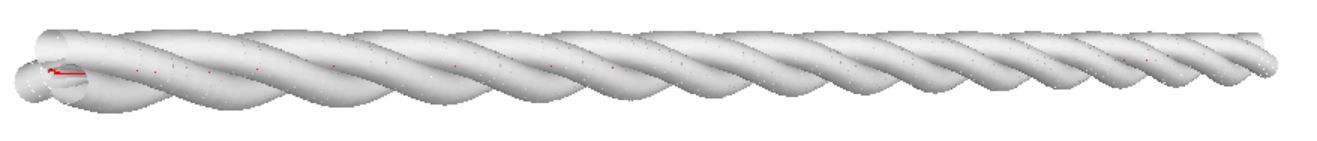
\includegraphics[width=.45\linewidth]{figures/lm_conductors}}\hfill
\subfloat[Armouring \label{fig:3phase}]
  {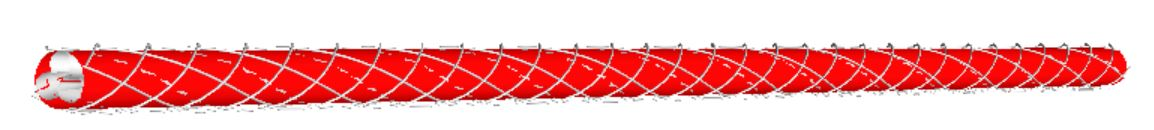
\includegraphics[width=.45\linewidth]{figures/lm_arm}}\hfill
\caption{Helical components in the local model}
\label{fig:local2}
\end{figure}





 



